ACH is currently being used as the primary IPC for the opensource BSD primary controller for the Hubo2 Plus (Hubo) full-size humanoid robot.  Hubo stands 130 $cm$ tall and weighs 37 $kg$ and has 2 arms, 2 legs and a head, thus it is anthromorphic to a human.  It bosts 38 degrees of freedom (DOF) consisting of: 6x in each leg, 6x in each arm, 5x in each hand, 1x in the weist, and 3x in the neck.

 Primary Hubo Controller (PHC) also knownfor the Hubo2 Plus full-size humanoid robots.  
The Hubo2 Plus is a 130 $cm$ tall humanoid robot commonly referred to as Hubo.  
Hubo weighs 37 $kg$ and has 40 DOF.
Each DOF, with the exception of the fingers, are high gain PD position controlled .  
There are 12 DOF in each leg, roll, pitch and yaw in the hip, pitch in the knee and roll and pitch in the ankle.  

The PHC runs on the concept of using separate process for 


\begin{figure}[thpb]
  \centering
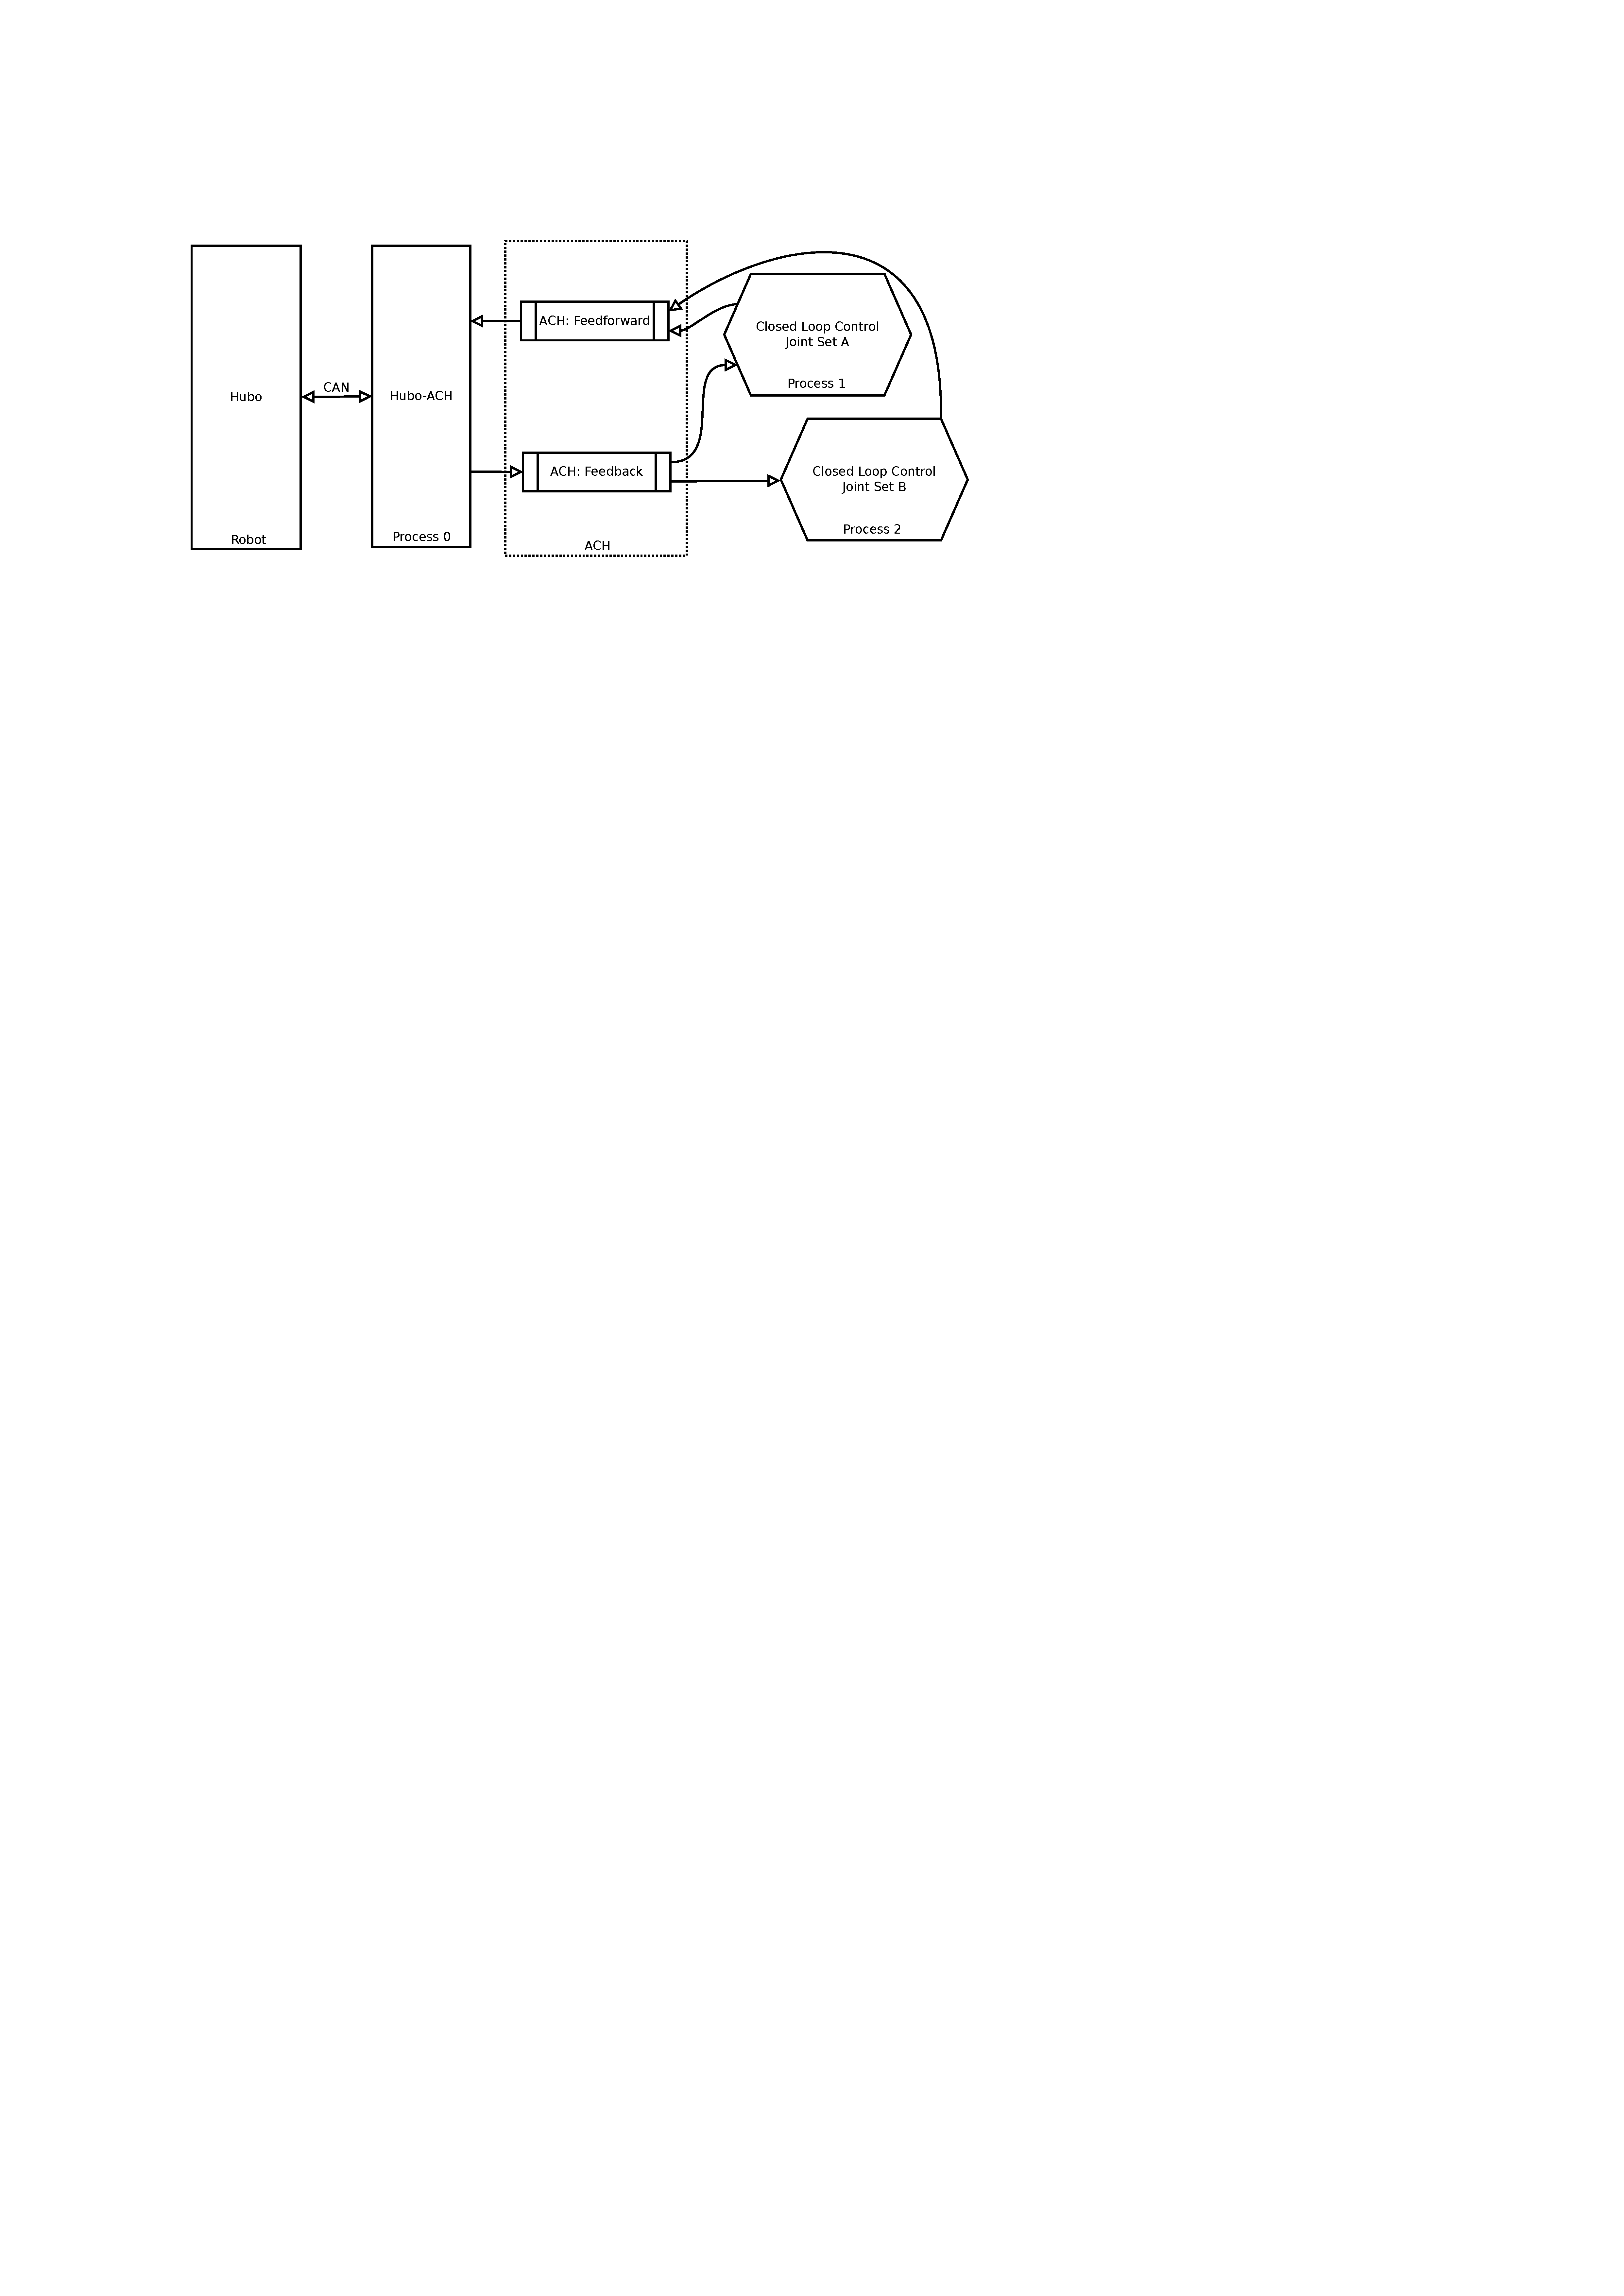
\includegraphics[width=1.0\columnwidth]{./pix/hubo-ach-diagram.pdf}
  \caption{Hubo Primary Controller (HPC) and system framework}
  \label{fig:graph}
\end{figure}

The primary PHC process is a daemon that talks over the CAN bus to all of the Hubo motor drivers and sensors.  
The \textit{feedforward} and \textit{feedback} states are stored in the \textit{HUBO\_REF\_CHANNEL} and \textit{HUBO\_STATE\_CHANNEL}.  
All information is stored in SI units.  The \textit{HUBO\_REF\_CHANNEL} holds a strut that has the desired reference for each of the joints in $rad$.  
The \textit{HUBO\_STATE\_CHANNEL} contains the sensor data and that joint status data.  
This includes:

\begin{itemize}
                \item Encoder position (rad), at each joint
                \item IMU x angle (rad), at CoM
                \item IMU y angle (rad), at CoM
                \item IMU Vx velos(rad/sec), at CoM
                \item IMU Vy velos(rad/sec), at CoM
                \item FT Mx moment (Nm), in Feet
                \item FT My moment (Nm), in Feet
                \item FT Fz force (N), in Feet
                \item Angle from acc Ax (rad), in Feet
                \item Angle from acc Ay (rad), in Feet
                \item G-force acc Az (G), in Feet
\end{itemize}

The PHC daemon runs in real-time using the preempt-rt kernel.  
All sensors are polled and motor references are set at the system period.  
This period is currently set to 0.004 $sec$, $T_H$.  
This period is limited by the bandwidth of the CAN communications bus which is currently set to 1.0 $Mbps$.  
Currently there are two CAN channels with one controlling the upper body and one the lower body.  
The operation frequency can be increase if more CAN channels are added.  
The PHC system is designed for ease of adding communication busses.  

At the beginning of each cycle the new references are set to each actuator.  
After each cycle the state is updated with the new sensor data.

A separate process will subscribe to the \textit{feedforward} and \textit{feedback} channels and run it's own real-time loop.  
This can run, update reference and read the feedback channel at any desired frequency within the processor and IPCs capabilities.
The PHC will always take the most recent reference from the feedforward channel at the rising edge of it's clock cycle with the period of $T_H$.
This ensures the motor drivers are updated at a constant rate. 
Each motor driver accepts a position reference and uses a phase locked loop (PLL) to lock onto the frequency and timing of the incoming reference commands.
The motor driver then linearly interpolates the reference commands from the current position to the set position to increase the commanded rate to the motor itself by 5 times the command frequency, $\frac{1}{T_H}$.
This is done to reduce the jerk of each of the actuated joints.

The key point is that the PHC runs with a period of $T_H$ and updates the motors with the references from the feedforward channel no matter what rate the external controller is updating the feedforward channel at.  
The sensors are also updated at a period of $T_H$.
The structure of the system can be found in Fig.~\ref{fig:graph}.

\begin{figure}[thpb]
  \centering
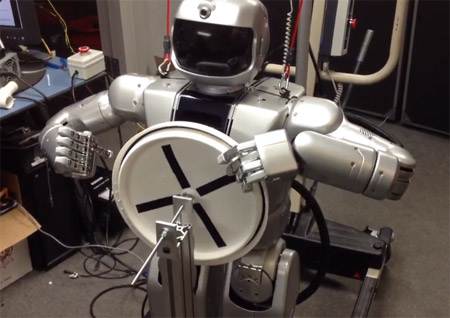
\includegraphics[width=1.0\columnwidth]{./pix/hubo_valve.png}
  \caption{Hubo running PHC turning a valve using trajectories created using Bi-RRTs. }
  \label{fig:valve}
\end{figure}

Current capabilities of the PHC system includes:

\begin{itemize}
\item Full Hubo2 Plus compatibility 
\item ROS support
\item Independent process for controllers
\item OpenRAVE trajectory playback
\item OpenHUBO integration 
\item Low frequency joint update filter.
\end{itemize}




